\documentclass[12pt]{article}

\usepackage[spanish]{babel}
\selectlanguage{spanish}
\usepackage[utf8]{inputenc}
\usepackage{vmargin}
\usepackage{graphicx}
\setmargins{2.5cm}{1.5cm}{16.5cm}{23.42cm}{0pt}{1cm}{0pt}{2cm}

\title{Análisis de Mareas}
\author{Martín Alejandro Paredes Sosa}
\date{Mayo 2015}
\graphicspath{{IMG/}}


\begin{document}
\maketitle

\section{Introducción}
En esta actividad se analizó un conjunto de datos de un sensor que mide: Fecha, tiempo, presión, temperatura del agua, nivel del mar y día del año. Los datos fueron proporcionados por el Dr. Julio César Rodríguez. Los datos se proporcionan en un archivo en formato de Excel, los cuales corresponden al manglar ``El Sargento". 

	La marea es el cambio periódico del nivel del mar producido principalmente por la fuerza de atracción gravitatoria que ejercen el Sol y la Luna sobre la Tierra. Sin embargo, hay que indicar que las mareas de la litosfera son prácticamente insignificantes, con respecto a las que ocurren en el mar u océano que pueden modificar su nivel en varios metros.
	
	Otros fenómenos ocasionales, como los vientos, las lluvias, el desborde de ríos y los tsunamis provocan variaciones del nivel del mar, pero no pueden ser calificados de mareas, porque no son causados por la fuerza gravitatoria.

\section{Historia}
El estudio de las mareas se remonta a los tiempos de Selecos de Seleucia (alrededor de 150 a.C.) que propuso que las mareas eran causadas por la Luna. Johannes Kepler, sugirió que la gravedad de la Luna causaba las mareas. Sin embargo, fue Isaac Newton fue el primero en explicar las mareas como resultado de la atracción gravitacional de masas astronómicas. Científicos famosos como Bernoulli, Euler,Maclaurin, Laplace, Thomson, Kelvin y Pioncare también contribuyeron a los avances sobre la teoría de mareas y sus comportamientos.
\begin{center}
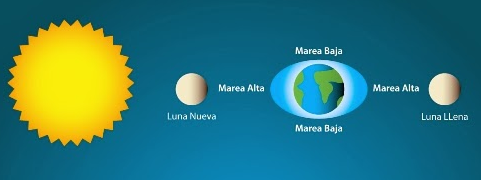
\includegraphics[width=10cm]{1mareas.png}
%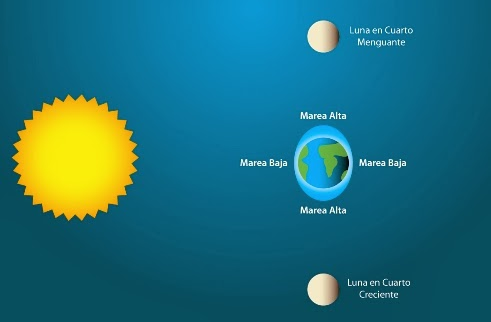
\includegraphics[width=7cm]{mareas1.png}
\end{center}

\pagebreak
\section{Teoría}
Los cambios de las tienen un orden
\begin{itemize}
\item El nivel del mar se eleva por varias horas.
\item El agua alcanza su nivel más alto, a lo que se conoce como marea alta.
\item El nivel del mar cae por varias horas.
\item El agua alcanza su nivel mas bajo, a lo que se conoce como marea baja.
\end{itemize}

Existen tres tipos de mareas:
\begin{description}
\item[Semidiurnas]: Se alcanzan dos mareas altas casi iguales y dos mareas bajas cada día.
\item[Diurna]: Se alcanza una marea alta y una baja.
\item[Mixta]: Se alcanza dos mareas desiguales cada día, o a veces una alta y una baja cada día. 
\end{description}
\begin{center}
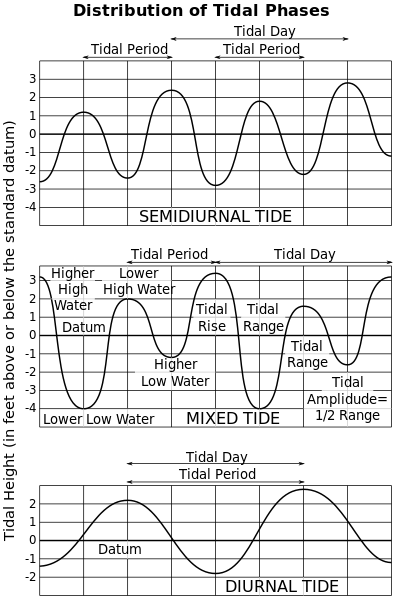
\includegraphics[height=10cm]{Tide_type.png}
\end{center}

\pagebreak

\section{Análisis de Datos}
Para la realización del análisis de los datos, se recurrió a la realización de un programa en FORTRAN Con el cual se leyeron los datos y se genero varios archivos con los cuales, usando GNUPLOT, se pueden graficar las mareas, sus puntos máximos y mínimos. Ademas de que se obtiene los periodos de las mareas.
\subsection{Código}
Con el siguiente código se realizo el análisis de datos
\begin{verbatim}
Module Conteo

  Implicit None
  Integer, Parameter :: Dat=7632 !Numeros de datos Totales
  Integer, Parameter :: Mes=1440 !Datos en un Mes
  Integer, Parameter :: Dias=159 !Numero de dias
  Integer, Parameter :: Day= 48  !Datos en un Dia
  Integer, Parameter :: Mdia=24  !Datos en medio dia
  Integer, Parameter :: MCo=5760 !Datos de los meses Completos

End Module Conteo

Program Periodos
  
  Use Conteo
  Implicit None
  Real,Dimension(Dat) :: T, Alt, Doy, Dyt, PeM, PeD, PeMD
  Real:: Maxm, Tmaxm, Minm, Tminm  
  Real:: Maxd, Tmaxd, Mind, Tmind
  Real:: Maxmd, Tmaxmd
  Real,Dimension(1:5):: Ti, Al
  Real, Dimension(1:Dias):: Tie, A
  Real, Dimension(1:2*Dias):: Tim, Hei
  Integer:: i, j

  Open(2, File="Mareas.csv")
  Open(3, File="Marea.dat", Status="Replace")
  Do i=1, Dat, 1
     Read(2,*) T(i), Alt(i), Doy(i), Dyt(i)
     Write(3,2) Dyt(i), Alt(i)
  End Do
  Close(2)
  Close(3)
  
  !Claculo de Maximos y Minimos por mes  
  Open(4, File="MaxMes.dat")
  Open(8, File="MinMes.dat")
  Do j=0, MCo, Mes
     Maxm=-1
     Do i=1, Mes, 1
        If(Alt(i+j)>Maxm) Then
           Maxm=Alt(i+j)
           Tmaxm=Dyt(i+j)
        End If
     End Do
     Write(4,2) Tmaxm, Maxm
  End Do

  Do j=0, MCo, Mes
     Minm=0
     Do i=1, Mes, 1
        If(Alt(i+j)<Minm) Then
           Minm=Alt(i+j)
           Tminm=Dyt(i+j)
        End If
     End Do
     Write(8,2) Tminm, Minm
  End Do
  Close(4)
  Close(8)
!Calculo de Maximos y Minimos por dia
  Open (5, File="MaxDias.dat")
  Open (9, File="MinDias.dat")
  Do j=0,Dat-1 , Day
     Maxd=-1
     Do i=1, Day, 1
        If(Alt(i+j)>Maxd) Then
           Maxd=Alt(i+j)
           Tmaxd=Dyt(i+j)
        End If
     End Do
     Write(5,2) Tmaxd, Maxd
  End Do

  Do j=0, Dat-1, Day
     Mind=0
     Do i=1, Day, 1
        If(Alt(i+j)<Mind) Then
           Mind=Alt(i+j)
           Tmind=Dyt(i+j)
        End If
     End Do
     Write(9,2) Tmind, Mind
  End Do

  Close(5)
  Close(9)
!Calculo de periodos

  Open(6, File="MaxMes.dat")
  Open(7, File="MaxDias.dat")
  Open(10, File= "Salida Principal.dat")
  
  Do i=1,5, 1 
     Read(6,*) Ti(i), Al(i)
     If(i>1) Then
        PeM(i)= Ti(i)-Ti(i-1)	
     End If
  End Do
  Write(10,*) "Ciclo Lunar:",Sum(PeM)/4 , "Dias"


  Do i=1 , Dias, 1
     Read(7,*) Tie(i), A(i)
     If(i>1) Then
       PeD(i)=Tie(i)-Tie(i-1)
     End If
  End Do

  Write(10,*) "Marea Diurna:", (Sum(PeD))/(Dias-1), "Dias"

 Close (6)
 Close (7)

!Calculo para mareas Semidiurna
 Open(11, File="SDiurna.dat")
  
 Do j=0, Dat-1, MDia
  Maxmd=-1
  Do i=1, Mdia, 1
    If(Alt(i+j)>Maxmd) Then
      Maxmd=Alt(i+j)
      Tmaxmd= Dyt(i+j)
    End If
  End Do
  Write(11,2) Tmaxmd, Maxmd
 End Do

 Close (11)
 Open(12, File="SDiurna.dat")
 !Calculo Periodo SDiurna
 Do i=1, 2*Dias, 1
   Read(12,*) Tim(i), Hei(i)
   If(i>1) Then
     PeMD(i)=Tim(i)-Tim(i-1)
   End If
 End Do
 Write(10,*) "Marea Semidiurna:", Sum(PeMD)/((2*Dias)-1), "Dias"
 
 Close (10)
  2 Format(2F10.2)
End Program Periodos
\end{verbatim}
\pagebreak

\subsection{Resultados del Análisis}
Los siguientes resultados fueron obtenidos de los datos  proporcionados por el Dr. Julio Rodriguez.
\begin{table}[h!]
   \centering
  \begin{tabular}{|p{5cm}|p{6cm}|}
  \hline
   & Periodo  \\   \hline
   Marea Semidiurna & 11 Horas y 58.8 minutos \\\hline
   Marea Diurna & 1 Día y 5.6 minutos\\\hline
   Ciclo Lunar & 29 Días y 6 horas\\\hline
    \end{tabular}
   \label{T2}
\end{table} 
\begin{center}
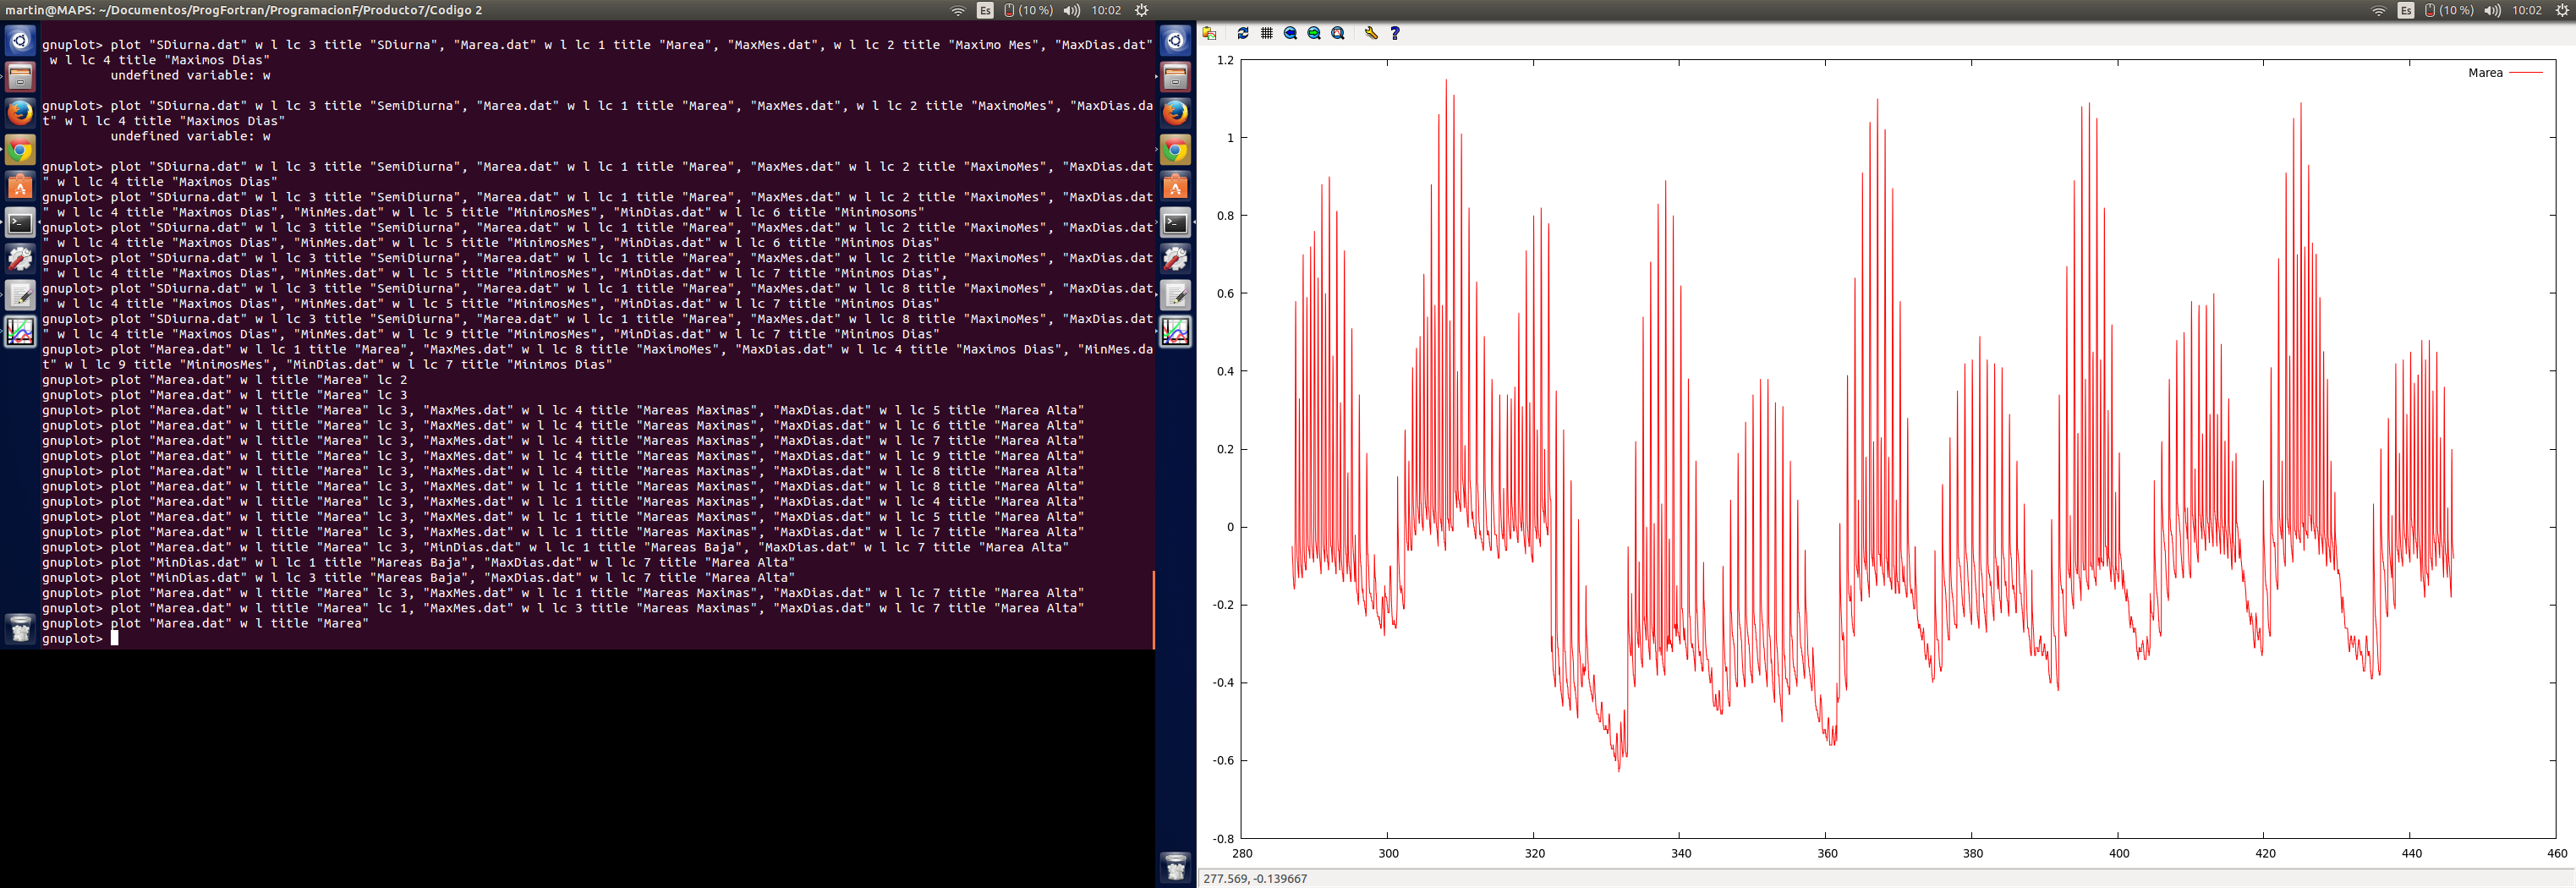
\includegraphics[width=15cm]{Marea.png}
%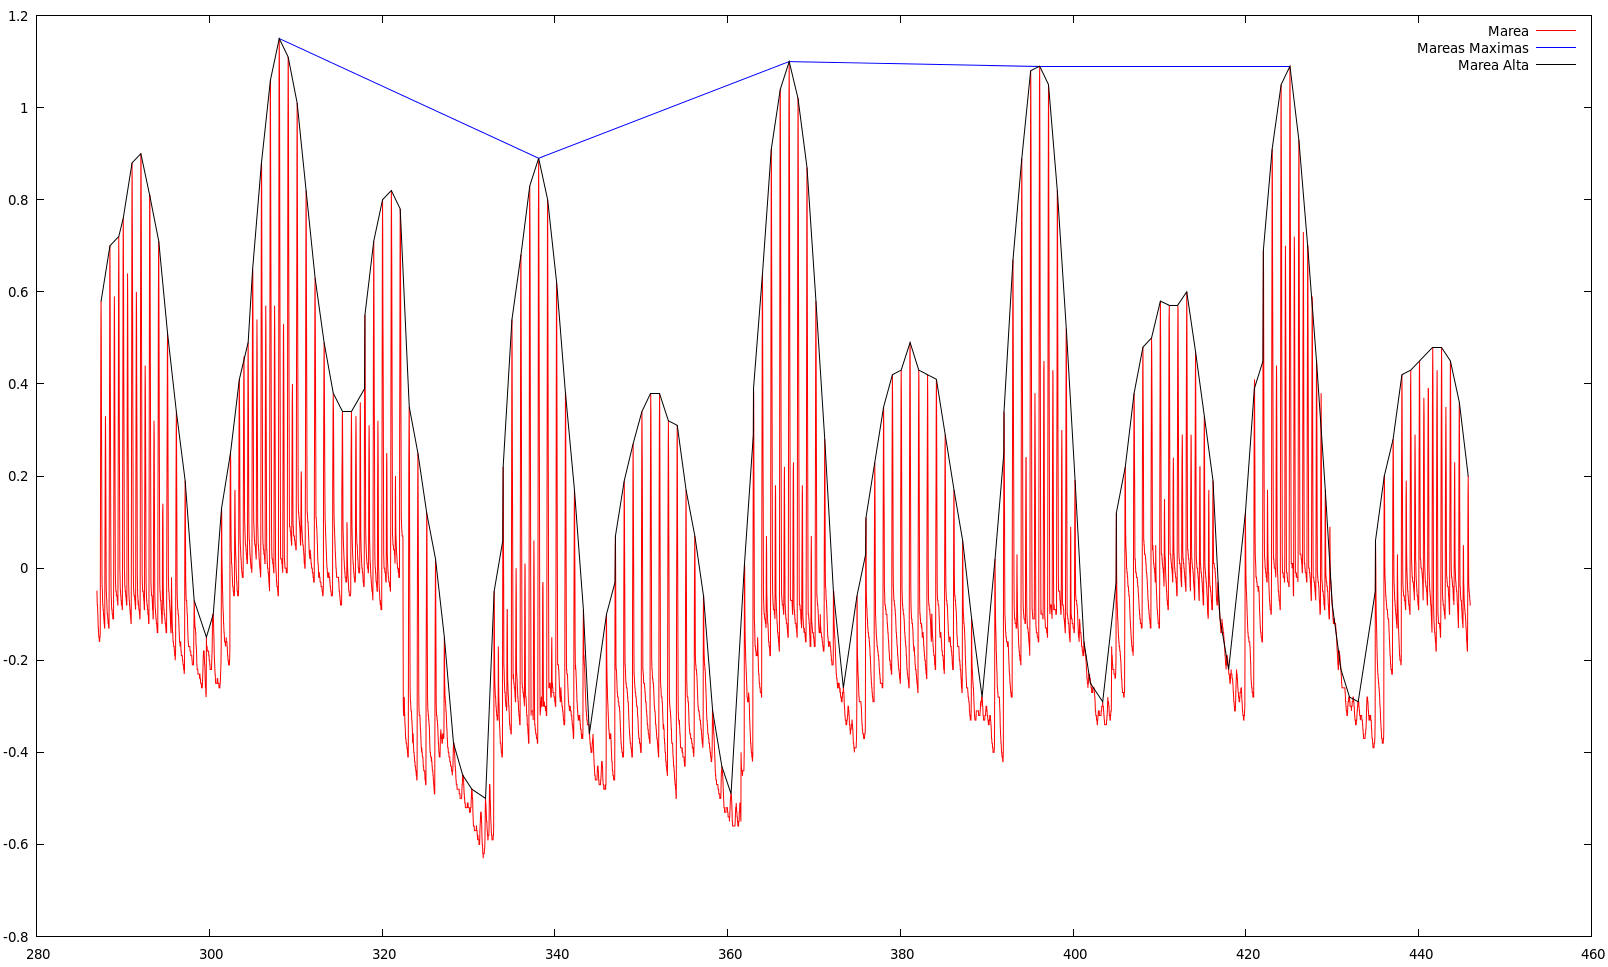
\includegraphics[width=15cm]{MareaMax.png}
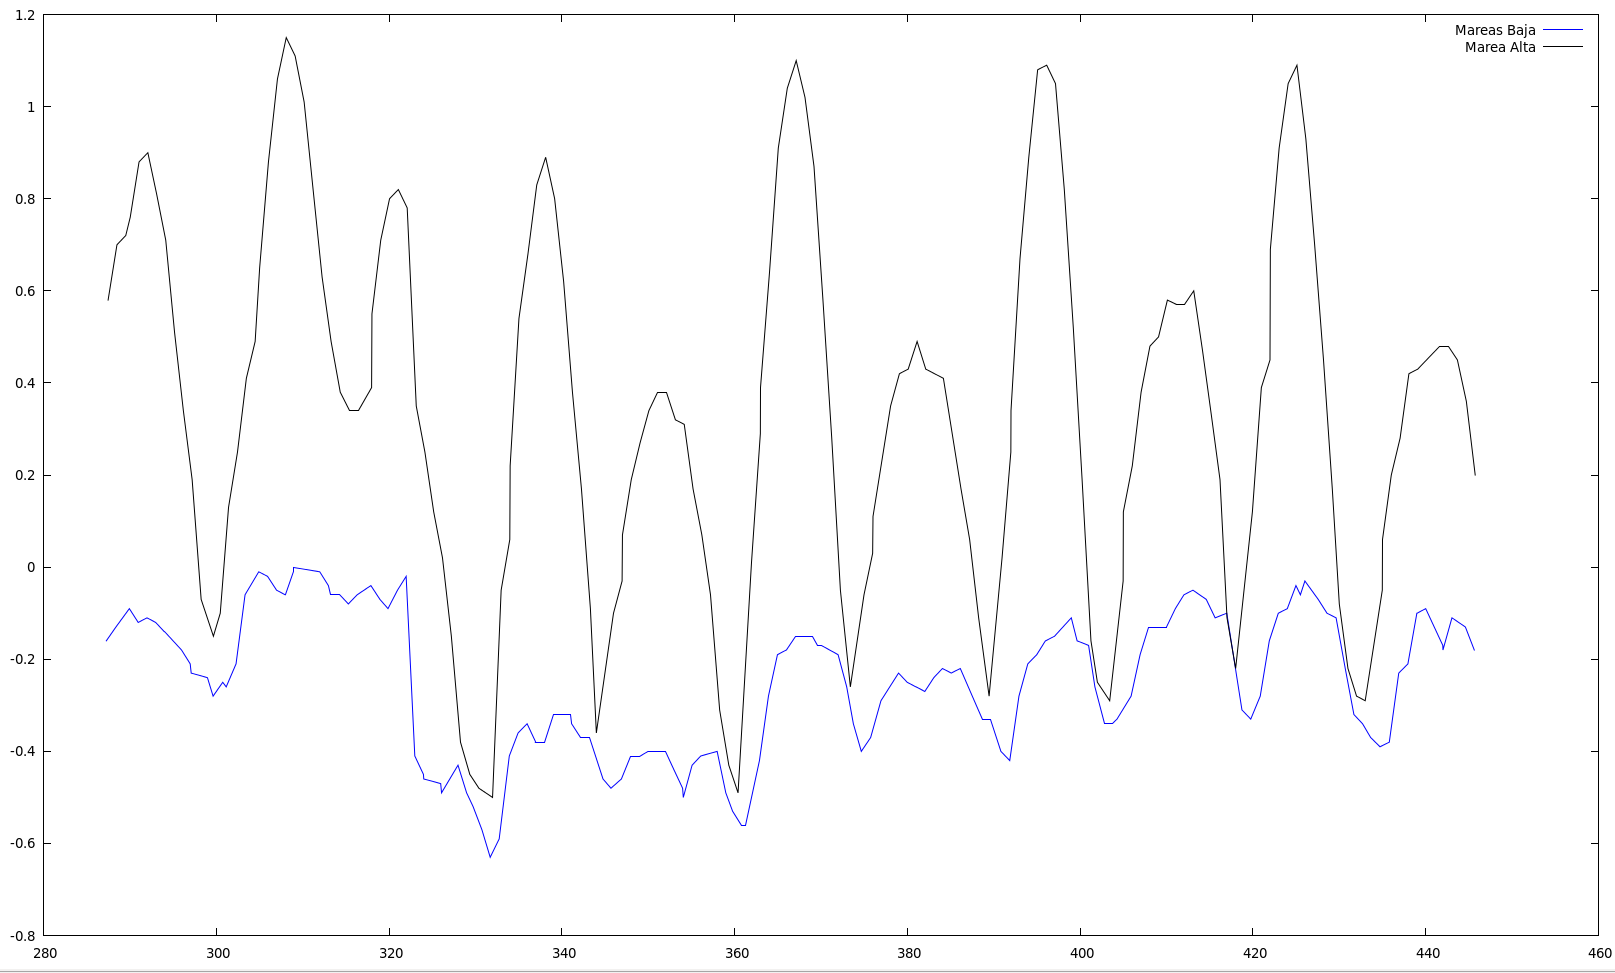
\includegraphics[width=15cm]{MareaMm.png}
\end{center}
\pagebreak
\section{Conclusión}
Los cambios en los niveles del mar a lo largo del día tiende a variar ya que esta no es igual a lo largo del mes debido a que el periodo no permite que ocurra a la misma hora. Gracias a esta información se pueden hacer predicciones y diversos cálculos con eventos que estén ligados a los cambios de la marea. 

\end{document}

